\chapter{\label{ch:6-evaluation} Evaluation}

%\minitoc

\section{Introduction}
A well documented issue with Natural Language Generation and other methods for generating prose is the problems with evaluating such systems. It can be hard to extract statistical data about how natural or believable the language sounds as well to derive performance measures for such a system in a way you could with other systems such as machine learning algorithms with more obvious relevant performance measures such as time and space complexity and measures of accuracy. These are not particularly useful in the case of a NLG system where an output being created in a reasonable amount of time is sufficient.\\

The majority of my evaluation was planned to be on the review of comments and replies observed on twitter and the blogging website, and a separate scenario where the believability of review generated is asked for in a test environment against real movie reviews gathered from the internet.

\section{Markov Chain text generation}
This was used as my baseline for generating movie prose, although it definitely served to be the least feasible of all the methods used. This was because the chains mostly produced complete nonsense when the corpora was expanded or the number of words represented as a node in a chain were decreased.\\
From my own observations, the text generated seemed more likely to be coherent at larger numbers of words per point in the chain, but were much more likely to form linear chains and copy text from the corpora verbatim, instead of producing something new. Smaller word counts would produce more original texts but would lose coherence much more quickly and fall apart much more quickly over larger output texts.

\section{Engagement With Twitter Bot}
The Twitter bot produced posts generated from Markov chains formed from corpora of tweets produced from twitter searches for terms related to certain movies. Every other tweet attempted to promote the blog website's hosted reviews.

\subsection{Results}
While the bot was running between the 17th of April to the 11th of May - a 25 day period - the tweets made generated a total of 13500 impressions. An impression is defined as any time a user has seen a tweet on Twitter.\\
An average of 551 impressions per day has been achieved while the bot has been running, although this has not amounted to a great amount of qualitative data - which is what I had hoped to obtain. The Twitter bot received very little attention in terms of link-clicks, follows and likes, even with hash tags for popular or controversial movies being used. A total of 34 link-clicks were obtained over this period, which is a very small amount relative to the number of overall engagements or impressions made over the time period. There were no real interactions with the bot outside of being followed by 3 other automated twitter accounts, all but one of which has since unfollowed. Occasionally words would trigger other bots to retweet them, but no human-controlled interactions were observed. \\
\begin{figure}
	\centering
	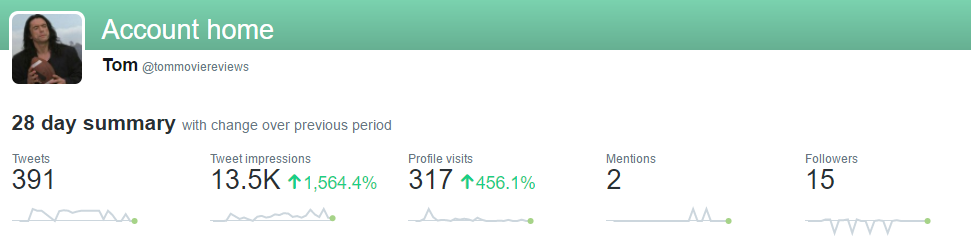
\includegraphics[width=0.7\linewidth]{figures/twitter_analytics/28daysummary}
	\caption[Summary of the past 28 days during which the bot was active]{}
	\caption{}
	\label{fig:28daysummary}
\end{figure}

\begin{figure}
\centering
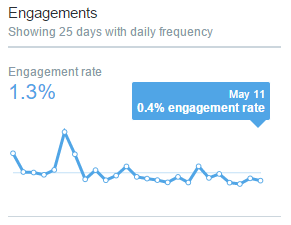
\includegraphics[width=0.7\linewidth]{figures/twitter_analytics/engagements}
\caption{Engagements with tweets made by the bot}
\label{fig:engagements}
\end{figure}

\begin{figure}
\centering
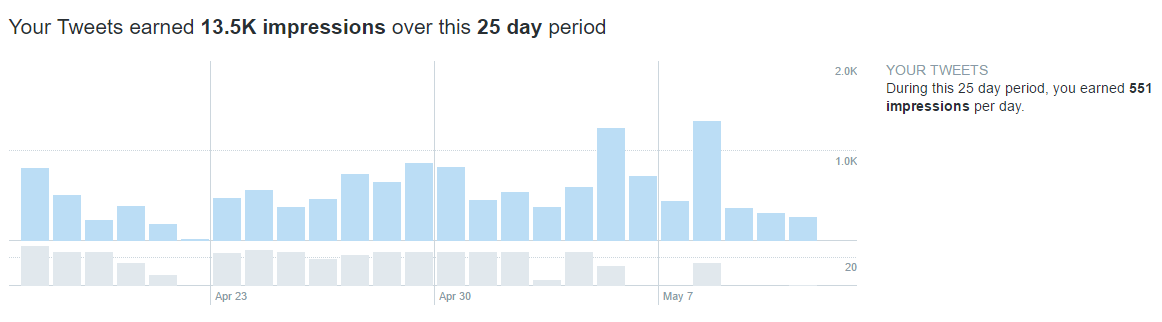
\includegraphics[width=0.7\linewidth]{figures/twitter_analytics/impressions}
\caption{Impressions had from the tweets made by the bot over 28 days}
\label{fig:impressions}
\end{figure}


\subsection{Observations}
The Twitter bot did not directly interact with any twitter users other than making posts, which may have limited the effect of its outreach. It would be interesting to implement post-liking or replying behaviours in the bot at a later date and see if that has an increased impact on the attention it receives. As well as this, the URL of the blog website may have been offputting towards potential readers and could have had an impact on the number of link clicks I have observed.\\
I would not say the bot was greatly successful in generating attention for the review website, due to the low number of link clicks had, but it did attract a small amount of attention using these relatively simple generative techniques.


\section{Comments and Interaction with Blog Website}
A number of reviews generated through the template system were hosted on the blog website, in order to see if they would receive any replies or feedback at all. This was later expanded to include reviews from the NLG system as well once that was implemented. It consists of an index page which loads a paginated list of movie reviews with a shortened preview of the article written with a link to the full text. The full text displays with a comments section below it.

\subsection{Results}
Unfortunately, there were no comments were left on the blog website, which is a shame as it would have been an interesting measurement of the believability of the reviews. Google analytics has however observed 53 unique sessions over the month the bot was active, involving 39 users generating 123 pageviews. The average number of pages visited in a session is 2.32 which indicates that users will have attempted to read at least one review, and clicked on to the homepage to view the rest of the site. The average session duration was 57 seconds, which indicates that at least some of the users stuck around long enough to attempt to read a review, although not all of them will have.\\
\begin{figure}
\centering
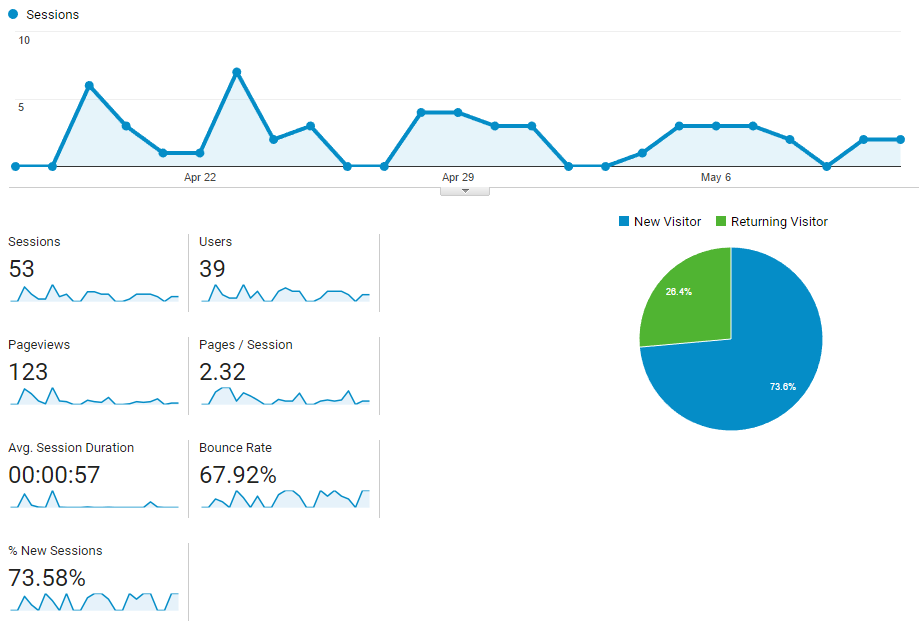
\includegraphics[width=0.85\linewidth]{figures/google_analytics/uniqueSessions}
\caption{Diagram of unique sessions held on the blog website.}
\label{fig:uniquesessions}
\end{figure}

\begin{figure}
\centering
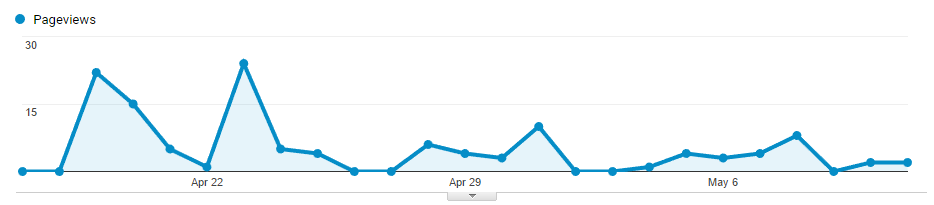
\includegraphics[width=0.85\linewidth]{figures/google_analytics/pageviews}
\caption{Pageviews during the time the blog website ran}
\label{fig:pageviews}
\end{figure}
\begin{figure}
\centering
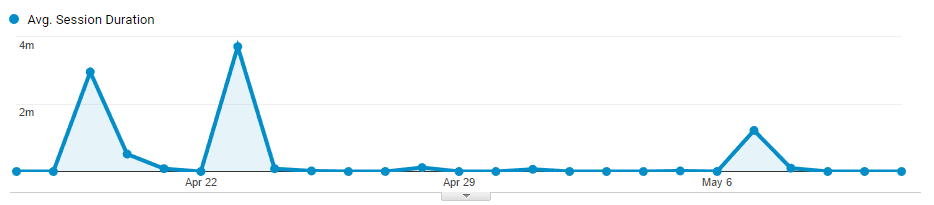
\includegraphics[width=0.85\linewidth]{figures/google_analytics/sessionDuration}
\caption{Average session duration over the life of the blog website}
\label{fig:sessionduration}
\end{figure}

\subsection{Observations}
I believe that a small, but not great amount of success was had from the Twitter bot generating this many unique sessions, although a failure of the content to be engaging enough to generate comment and feedback.\\
It is a valid criticism that the hosting of the website on the Department of Computing servers could throw people off from following the link and interacting with the website, as it is not a tidy URL (doc.gold.ac.uk/~tpalm003/reviews/index.php vs. something like tomsreviews.com) with an easily recognisable domain.\\
Another criticism is that the design of the blog is fairly simplistic and that its design may not be as convincing as other blog platforms for hosting movie reviews because of this.\\


\section{Turing Test Scenario}
In order to collect more detailed feedback on the NLG system, I set up a Turing-like test. Users were shown sentences and full reviews which were generated via the NLG system implemented, as well as real sentences and full reviews written by IMdB users. These were ordered randomly, and 4 examples of each case were selected. The users were shown these in a randomized order so there were no contextual clues as to whether or not the review was human or not, although the order that each user is shown the data was the same.

\subsection{Results}
I was able to obtain a good amount of feedback on the NLG system through this system. 11 respondents participated in the test (and 9 provided feedback for each of the examples given) and I managed to obtain interesting data on how the NLG system performs on the sentence and full text levels.\\
Generally, people found the full review texts that were generated to be less coherent and less human-like than real reviews, although the first review they were shown that was generated was received as coherent by 7 of the 11 respondents, and believably written by a human by 5, this effect wore off as they were shown more reviews and their structure was noticed. The final generated review seen was only thought to be human by 2 of the respondents, although voted coherent by 5 of 9 who made it to the end of the feedback session. \\

One user wrote "after you've read a couple of these the pattern becomes very obviously robotic," which demonstrates the point that the text generated follows a structure that is easy to recognise over multiple examples.\\

On the sentence level, it became very hard for participants to tell the difference between a generated sentence and a sentence taken from a real review, where the difference in scores closed, although some users were able to tell a sentence was generated due to it's pattern being seen in previous examples of full reviews. Generated sentences generally scored 8 out of 11 for how human they were each time, and between 5 and 7 out of 11 for their coherence. In contrast, real sentences scored between 5 and 8 out of 11 for how human they appeared, and 2 and 8 for how coherent they were. It is worth mentioning that I intentionally included sentences from less well written reviews in order to throw users off in terms of the exact way in which the reviews and sentences are generated by my system.\\
\begin{table}

\begin{center}
	\begin{tabular}{||c c c c c||} 
		\hline
		Position Seen & Text Type & Human & Coherent & Total Respondents \\ [0.5ex] 
		\hline\hline
		5 & NLG Review & 5  & 7 & 11 \\ 
		\hline
		10& NLG Review& 6& 5&10\\
		\hline
		13& NLG Review& 3& 6&9\\
		\hline
		15& NLG Review& 2& 5&9\\
		\hline
		3& NLG Sentence& 8& 6&11\\
		\hline
		7& NLG Sentence& 8& 7& 11\\
		\hline
		11& NLG Sentence& 8& 5&10\\
		\hline
		2& Real Paragraph& 5& 11& 11\\
		\hline
		6& Real Paragraph& 2& 10& 11\\
		\hline
		9& Real Paragraph& 7& 7&10\\
		\hline
		1& Real Sentence& 8& 2& 11\\
		\hline
		4& Real Sentence& 7&5&11\\
		\hline
		8& Real Sentence& 6& 7&11\\
		\hline
		12& Real Sentence& 5& 9&9\\
		\hline
		14& Real Sentence& 7& 8&9\\
		\hline
		16& Real Sentence& 6& 4&9\\		[1ex] 
		

		\hline
	\end{tabular}
\end{center}
\caption{Table displaying feedback provided on each excerpt, along with its type and order of appearance}
\end{table}

\subsection{Observations}
At the sentence level, it was difficult for readers to identify between the NLG system and real written reviews. However, this fell apart at the full review level when the initial review they read often failed to appear human-like and after more generated reviews were shown to them they also often became able to identify their structure and easily tell that they were generated through this.\\

The generation of sentences which convey sentiment and opinion seems to have gone well with the NLG system, where users struggle to tell them apart from real sentences. There is an issue with the variety of these sentences produced as some of the patterns and their handling are hard-coded and have flavour added to them from templates, as the data needed to form the actual opinion proved too difficult for me to extract.\\

It would appear that a weakness of the NLG system is the rigid document structuring that has been implemented, which seems to quite heavily impact the detection of these reviews over multiple documents. While this is less of a problem for single documents, it is certainly a worthwhile improvement to have more fluid and variable structures when generating documents to give the impression of a human author.\\
As well as this, another shortcoming of the NLG system is that to discuss a topic, data needs to be gathered on it to begin with. This is difficult in the case of discussing themes, plot synopses, tone and other higher concept topics that are discussed in reviews of art. An interesting area of improvement would be to implement some method for identifying and extracting data on some of these higher concepts from the review text corpora.


